\chapter{Conclusion}\label{chapter:conclusion}

\noindent For the validation of the first hypothesis, which states that using GraphQL with a common caching layer and a mechanism to reduce queries can prevent over-fetching and over-requesting, a micro-frontend architecture with four \acp{SPA} and eight widgets was designed and implemented. Before the implementation, the old legacy system was analyzed to identify potential bounded contexts that could be extracted into a separate micro-frontend. The prototype was implemented using mainly Angular and React for a single widget. The micro-frontends were integrated using client-side integration with the help of Webpack's Module Federation. A \ac{BFF} service in the form of a GraphQL \ac{API} was implemented using the dependency Apollo Server. This service provides a gateway for the interfaces of the microservices that live inside the company's service cluster. The \ac{BFF} takes care of fetching and aggregating the data from multiple microservice. The data from the microservices is later used for the GraphQL queries. The GraphQL \ac{API} was querying and mutating mocked datasets during development because the microservice cluster was not fully operational. The micro-frontend prototype will be integrated into the company's infrastructure sometime in the future and it will replace the legacy management system. Therefore, the GraphQL schema and queries will be used later in production, making the evaluations' results very expressive.

\bigskip

\noindent The first step was implementing a communication system where the application shell could communicate with the remote modules. The shared caching layer was implemented with the help of Angular's Dependency, which laid the groundwork for the communication pattern. To further improve the performance of the caching layer, a mechanism was implemented to provide the micro-frontend with the possibility to remove fields from GraphQL queries already stored inside the cache. This behavior is not natively implemented in Apollo Client, but the apollo-augmented-hooks library provided precisely that functionality. However, the library was outdated and lacked support for frameworks other than React. Therefore, the library was forked, and the functionality was made technology agnostic. Several new features have been added to further leverage the cache and remove unnecessary fields from a query.

\bigskip

\noindent Three distinct configurations for the applications were identified to compare whether the shared caching layer and the reduction of queries improve performance. The first approach is a naive approach with no shared caching layer and no reduction of queries. The second approach uses the shared caching layer but no reduction of queries. Furthermore, the third approach used the shared caching layer and the reduction of queries. Measuring and comparing the results of the measurements came with surprising results. The shared caching layer brought immense performance gains by significantly reducing the number of network requests and the total response size by multiple megabytes. However, reducing queries with the help of apollo-augmented-hooks functionality has not obtained the expected results. In contrast to the immense savings from the shared caching layer, reducing queries does not make a significant difference when comparing the request and response sizes. The additional functionality to reduce queries with the help of the cache brings additional complexity in the form of maintaining the functionality. Each new release of the \texttt{InMemoryCache} of Apollo could break the implementation, as the library directly depends on the cache's functionality. Changing the public \ac{API} might break the workflow of reducing queries. Another difficulty in using the query reduction mechanism is stale and inconsistent data. By fetching only fields not already in the cache, the data in the cache might become invalid. Especially for rapidly changing data, outdated and fresh data might be mixed in the same cache object. The Apollo Client provides fetch policies to handle data that is rapidly changing, but this makes the use of query reduction unnecessary. 
The use cases of the built prototype do not leverage the potential of query reduction. The prototype mainly consists of a list view and a detail view for data from the GraphQL \ac{API}. This scenario does not leverage the potential of query reduction because only a few fields are omitted from the queries. The list view mostly shows a handful of fields that can be reduced from the query. These fields mostly contain small fields.

\bigskip

\noindent Based on the discussion points, hypothesis I is partially confirmed. The number of requests and network traffic can be drastically reduced with the help of a shared caching layer. This approach is a simple and relatively implemented solution that brings enormous performance improvements. Nevertheless, using a mechanism to reduce queries with existing fields in the cache does not bring the desired performance improvements in the contexts of this prototype. The theoretical example above shows where query reduction circumvents the limitations of the Apollo Client and brings massive performance improvements.

\bigskip

\noindent Query reduction does not work well with the structure of fetching data inside the micro-frontend architecture, as explained before. Nevertheless, other applications might greatly benefit from such a mechanism. A great inconvenience of Apollo Client's cache is that when the same query is fetched two times and the second query contains one field that was not already in the first query, the query will always be executed against the GraphQL \ac{API}. The other way around works well. If a query contains only fields or a subset of the fields already inside the cache, the data for the query is populated just from the cache. Another inconvenience is that caching works just on the query level. The prototype mostly fetches part of the data inside a list view and the complete data inside a detail view. With the default behavior of Apollo Client, the query is always executed against the cache, because the query's name differs. The \texttt{InMemoryCache} does not know that the detail part data is already in the cache, because another query fetched it. The only solution for that problem is to define a cache redirect for every type, which is quite cumbersome.

\bigskip

\noindent To validate the second hypothesis, which states that the prototype should provide enough freedom in the choice of technology, a micro frontend was written using React and embedded in the shell application. Module Federation is a great tool that provides many options for integrating applications from various frameworks into the application shell. The application shell has implemented abstractions for integrating frameworks other than Angular into the unidirectional data flow. The React application integrated with the existing architecture and used both the shared caching layer and the query reduction mechanism. The architecture is thus theoretically open to the free choice of technology. However, it has to be considered that running multiple frontend frameworks on the same architecture leads to large bundle sizes, which negatively impact the performance of the client.

\ifshowImages
  \begin{figure}[H]
    \centering
    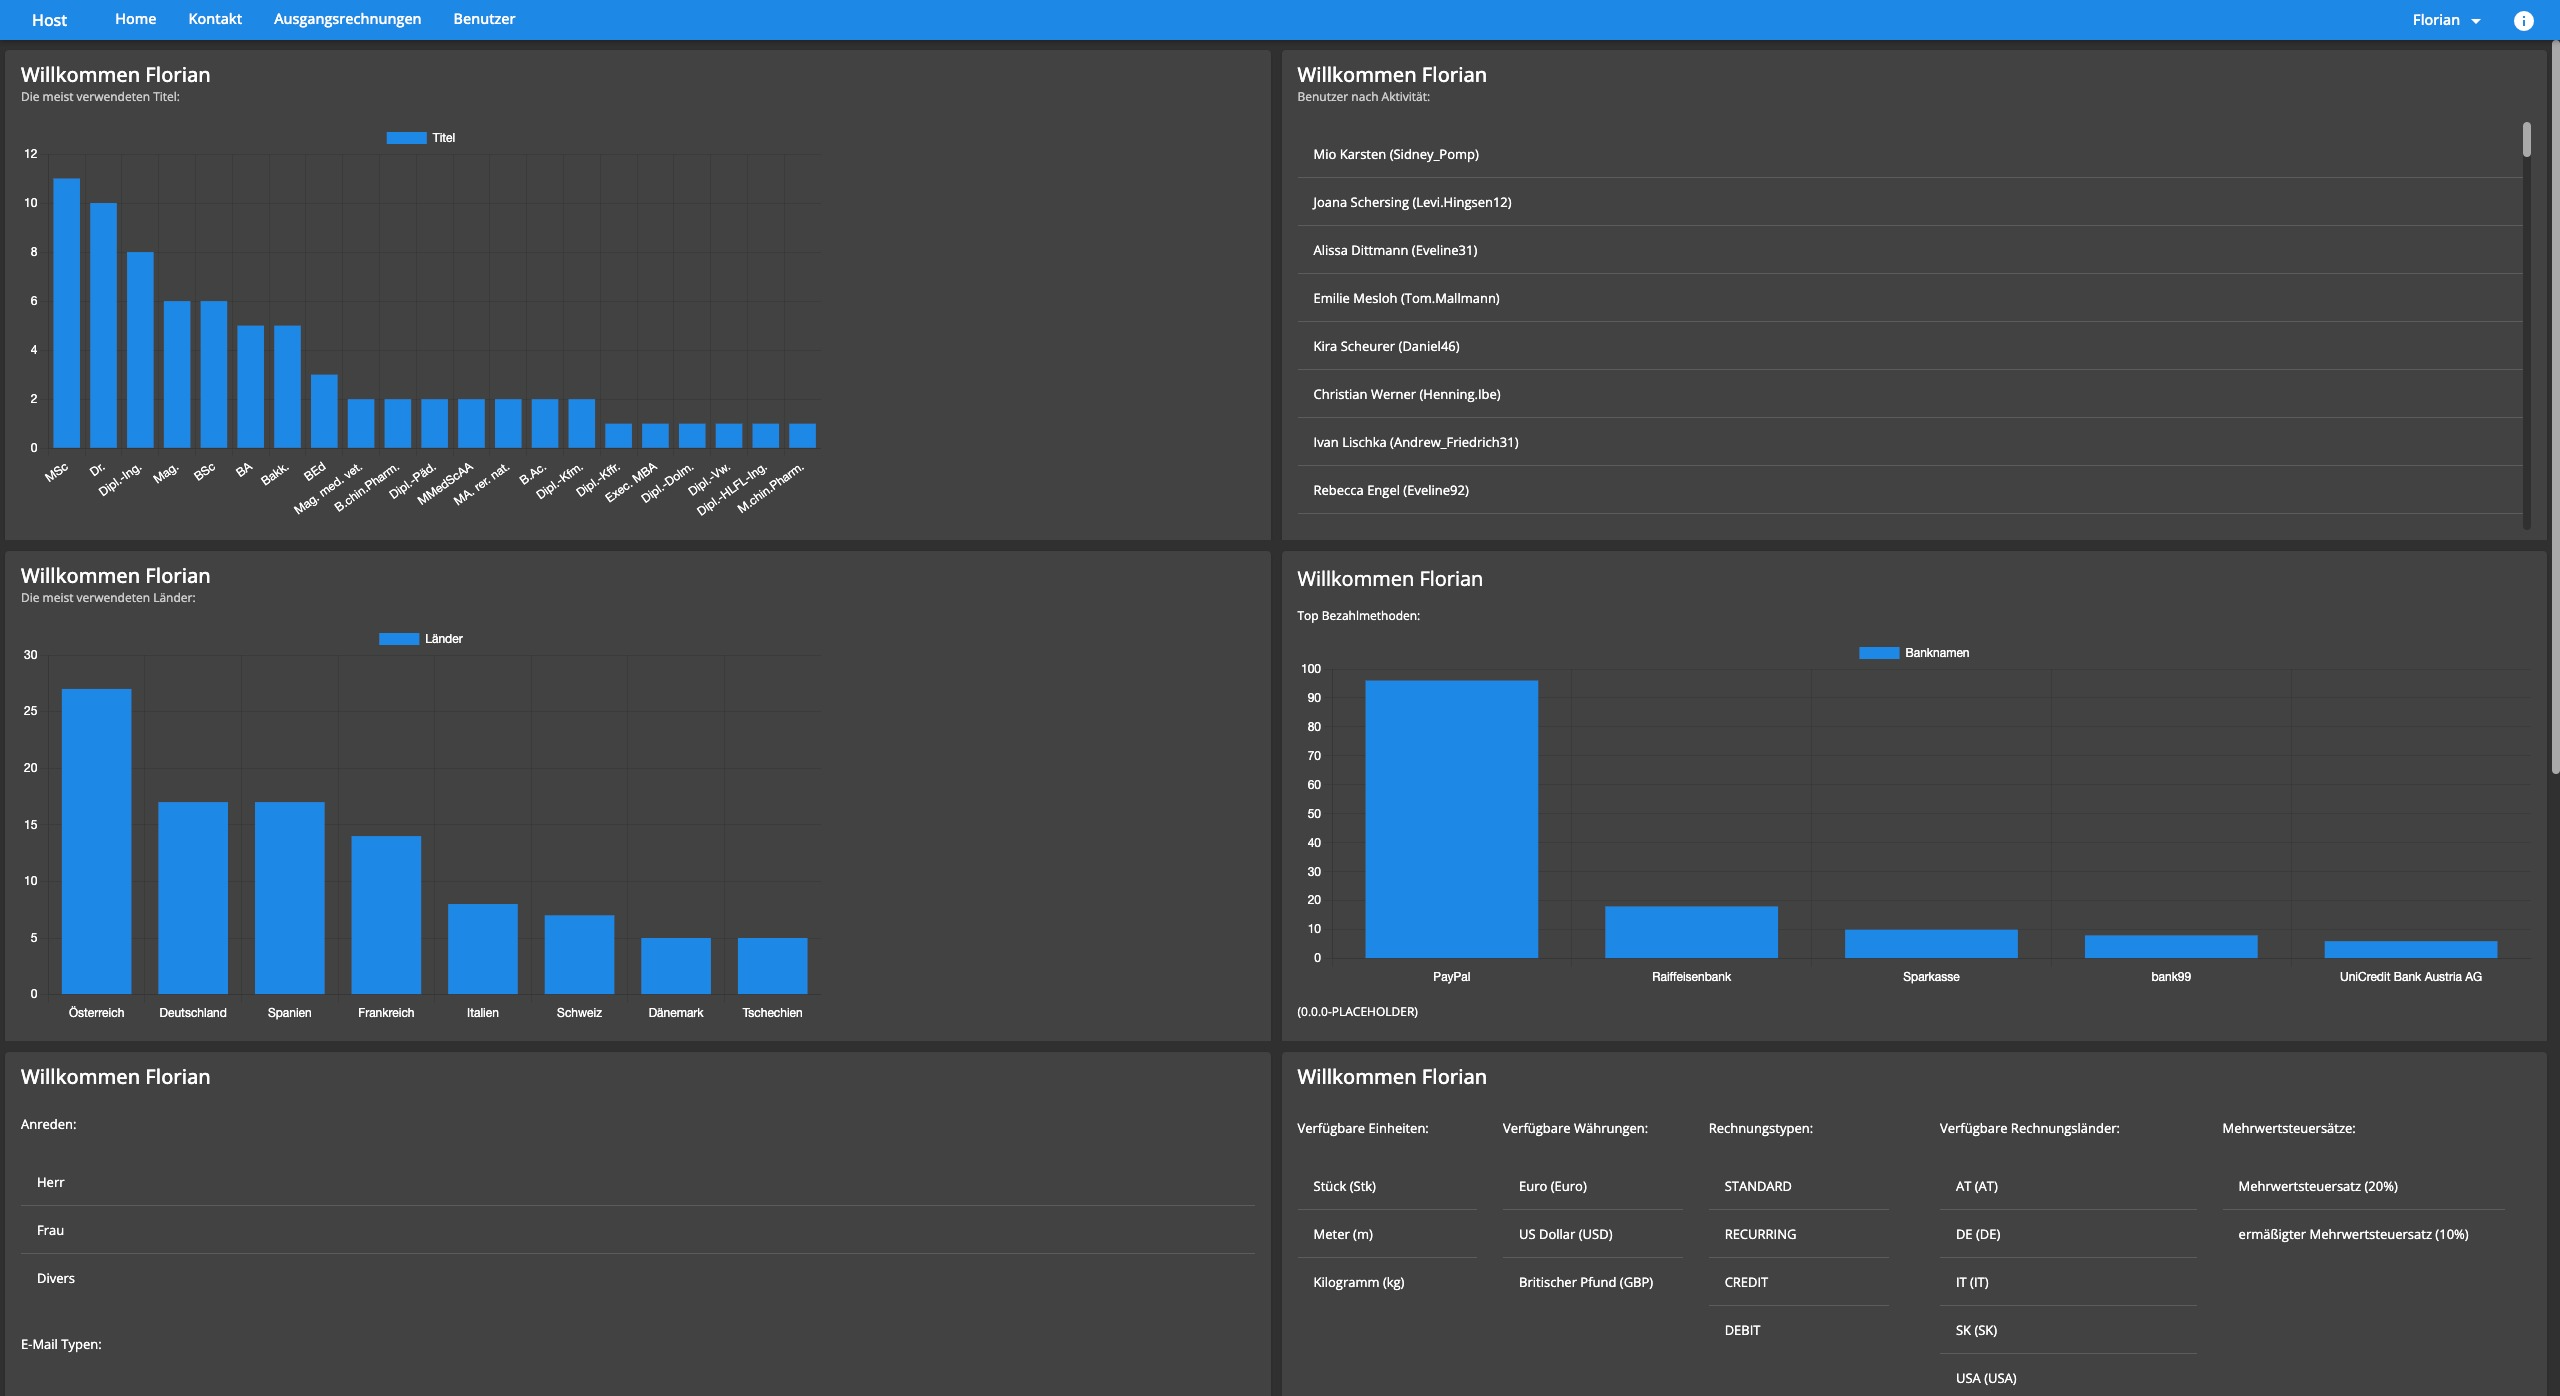
\includegraphics[width=1\linewidth]{images/prototype-screenshots/ui-dashboard.png}
    \caption{}\label{fig:conclussion:ui-dashboard}
  \end{figure}
\fi